\documentclass[12pt]{article}
\usepackage[utf8]{inputenc}
\usepackage[utf8]{vietnam}
% Enforce English captions while keeping Vietnamese character support
\AtBeginDocument{%
  \renewcommand{\contentsname}{Contents}
  \renewcommand{\listfigurename}{List of Figures}
  \renewcommand{\listtablename}{List of Tables}
  \renewcommand{\refname}{References}
  \renewcommand{\indexname}{Index}
  \renewcommand{\figurename}{Figure}
  \renewcommand{\tablename}{Table}
  \renewcommand{\partname}{Part}
  \renewcommand{\appendixname}{Appendix}
}
\usepackage{graphicx}
\usepackage{geometry}
\geometry{a4paper, margin=2cm}
\usepackage{amsmath}
\usepackage{amssymb}
\usepackage{booktabs} % For professional tables
\usepackage{listings}
\usepackage{xcolor}
\usepackage{caption}
\usepackage{float}
\usepackage[hyphens]{url}
\usepackage{ragged2e} % For better justification control
\usepackage[bookmarks=true, bookmarksopen=true, bookmarksnumbered=true, colorlinks=true, linkcolor=black, urlcolor=blue, citecolor=black]{hyperref}

\definecolor{codegreen}{rgb}{0,0.6,0}
\definecolor{codegray}{rgb}{0.5,0.5,0.5}
\definecolor{codepurple}{rgb}{0.58,0,0.82}
\definecolor{backcolour}{rgb}{0.95,0.95,0.92}

\lstdefinestyle{mystyle}{
    backgroundcolor=\color{backcolour},   
    commentstyle=\color{codegreen},
    keywordstyle=\color{magenta},
    numberstyle=\tiny\color{codegray},
    stringstyle=\color{codepurple},
    basicstyle=\ttfamily\footnotesize,
    breakatwhitespace=false,         
    breaklines=true,                 
    captionpos=b,                    
    keepspaces=true,                 
    numbers=left,                    
    numbersep=5pt,                  
    showspaces=false,                
    showstringspaces=false,
    showtabs=false,                  
    tabsize=2
}

\lstset{style=mystyle}

\begin{document}

\begin{titlepage}
    \centering
    {\large \textbf{UNIVERSITY OF SCIENCE AND TECHNOLOGY OF HANOI} \par}
    \vspace{4cm}
    
\includegraphics[width=0.6\textwidth]{usth.png} \par
    \vspace{3cm}
    {\Large \textbf{MACHINE LEARNING AND DATA MINING II} \par}
    \vspace{0.5cm}
    {\Large \textbf{LABWORK 3: CLASSIFICATION I} \par}
    \vfill
    {\large \textbf{TẠ HIẾU NAM (22BI13327)} \par}
    \vspace{0.3cm}
    {\large \textbf{ĐỖ DUY TOÀN (22BI13420)} \par}
    \vspace{2cm}
    \vfill
    {\large \textbf{Lecturer: Dr. Đoàn Nhật Quang} \par}
    \vspace{1.5cm}
    \thispagestyle{empty}
\end{titlepage}

\pagenumbering{roman}
\tableofcontents
\newpage
\listoftables
\listoffigures
\newpage

\pagenumbering{arabic}
\justifying

\section{K-nearest neighbor classification}

The objective of this section is to study the use of the K-Nearest Neighbor (K-NN) method for classification tasks.

\subsection{Select two datasets with labels}

Two distinct datasets were selected to evaluate the performance of K-NN:

\begin{enumerate}
    \item \textbf{Mice Protein Expression:} This biological dataset consists of 1080 samples with 77 continuous features representing protein expression levels. The target variable comprises 8 classes. The dataset contains some missing values which were handled via simple imputation.
    \item \textbf{ISOLET (Isolated Letter Speech Recognition):} This dataset contains speech data for 26 English alphabets (classes). The training set has 6238 samples and the test set has 1559 samples. Each sample is described by 617 continuous features.
\end{enumerate}

\subsection{Run K-NN on these two datasets and calculate classification error}

\subsubsection{Methodology and Algorithm Description}
The K-Nearest Neighbors (K-NN) algorithm is a non-parametric, instance-based learning method utilized for classification. For any given query point in the test set, the algorithm identifies the $k$ closest training examples in the high-dimensional feature space based on a specific distance metric. In this study, we employed the \textbf{Euclidean distance}, which is defined for two points $p$ and $q$ in an $n$-dimensional space as:
\begin{equation}
    d(p, q) = \sqrt{\sum_{i=1}^{n} (p_i - q_i)^2}
\end{equation}

Once the $k$ nearest neighbors are identified, the algorithm assigns the class label to the query point via a majority voting mechanism among its neighbors. We utilized the default parameter $k=5$, balancing the trade-off between noise sensitivity (which affects small $k$) and the smoothing of decision boundaries (which affects large $k$).

\subsubsection{Implementation Details}
The experiments were conducted using Python's \texttt{scikit-learn} library. The core implementation relies on the \texttt{KNeighborsClassifier} class. The workflow consists of:
\begin{enumerate}
    \item \textbf{Model Initialization:} \texttt{knn = KNeighborsClassifier(n\_neighbors=5)}
    \item \textbf{Training:} The \texttt{fit(X\_train, y\_train)} method stores the training data for efficient querying.
    \item \textbf{Prediction:} The \texttt{predict(X\_test)} method computes pairwise distances between test instances and stored training points to infer labels.
\end{enumerate}

\subsubsection{Performance Metric: Accuracy and Error calculation}
The primary metric for evaluation is \textbf{Classification Accuracy}, defined as the proportion of correctly classified instances. This can be expressed in two equivalent formulations:

\paragraph{Formulation 1: Indicator Function.}
\begin{equation}
    \text{Accuracy} = \frac{1}{N} \sum_{i=1}^{N} \mathbb{I}(\hat{y}_i = y_i)
\end{equation}
where $N$ is the number of test samples, $\hat{y}_i$ is the predicted label, $y_i$ is the ground truth label, and $\mathbb{I}(\cdot)$ is the indicator function that equals 1 when the condition is true and 0 otherwise.

\paragraph{Formulation 2: Confusion Matrix Components.}
Alternatively, accuracy can be expressed in terms of the confusion matrix:
\begin{equation}
    \text{Accuracy} = \frac{\text{TP} + \text{TN}}{\text{TP} + \text{TN} + \text{FP} + \text{FN}}
\end{equation}
where:
\begin{itemize}
    \item \textbf{TP (True Positives):} Instances correctly classified as belonging to a class.
    \item \textbf{TN (True Negatives):} Instances correctly classified as not belonging to a class.
    \item \textbf{FP (False Positives):} Instances incorrectly classified as belonging to a class.
    \item \textbf{FN (False Negatives):} Instances incorrectly classified as not belonging to a class.
\end{itemize}

For multi-class problems, these metrics are aggregated across all classes. The confusion matrices presented in Section 1.2.5 provide a visual representation of these components.

\paragraph{Implementation.} In practice, accuracy is computed using \texttt{sklearn.neighbors.KNeighborsClassifier} for model training and \texttt{sklearn.metrics.accuracy\_score} for evaluation. After training the classifier with \texttt{fit(X\_train, y\_train)}, predictions are obtained via \texttt{predict(X\_test)}, and accuracy is calculated by comparing predicted labels against ground truth labels.

Consequently, the \textbf{Classification Error} is derived as:
\begin{equation}
    \text{Error} = 1 - \text{Accuracy}
\end{equation}

\subsubsection{Experimental Results}
Upon applying this methodology to the two selected datasets, we obtained the baseline performance metrics summarized in Table \ref{tab:knn_baseline}.

\begin{table}[H]
\centering
\begin{tabular}{lccccc}
\toprule
\textbf{Dataset} & \textbf{Train Size} & \textbf{Test Size} & \textbf{Features} & \textbf{Accuracy} & \textbf{Error} \\
\midrule
Mice Protein & 756 & 324 & 77 & 92.59\% & \textbf{7.41\%} \\
ISOLET & 6238 & 1559 & 617 & 91.28\% & \textbf{8.72\%} \\
\bottomrule
\end{tabular}
\caption{Baseline K-NN performance ($k=5$) on both datasets.}
\label{tab:knn_baseline}
\end{table}

\paragraph{Analysis.} The initial results demonstrate that K-NN achieves competitive classification performance on both datasets without any preprocessing or hyperparameter tuning. For the \textbf{Mice Protein Expression} dataset, the algorithm correctly classified 92.59\% of test instances, yielding a classification error of 7.41\%. This indicates that the protein expression profiles exhibit sufficient discriminative power to separate the 8 biological classes based solely on local neighborhood information in the 77-dimensional feature space.

For the \textbf{ISOLET} dataset, despite the significantly higher dimensionality (617 features) and larger number of classes (26 letters), K-NN achieved a comparable accuracy of 91.28\% with an error rate of 8.72\%. This suggests that the spectral features extracted from speech signals form well-separated clusters in the high-dimensional space, allowing the distance-based voting mechanism to effectively distinguish between different phonemes.

\paragraph{Interpretation.} These baseline results validate the applicability of K-NN to both biological and speech recognition domains. The relatively low error rates (below 10\%) without any feature engineering suggest that:
\begin{itemize}
    \item The structure of both datasets aligns well with the K-NN assumption that similar instances belong to the same class.
    \item The Euclidean distance metric, while simple, captures meaningful similarity relationships in these feature spaces.
    \item The default choice of $k=5$ provides a reasonable balance between local sensitivity and noise robustness for both datasets.
\end{itemize}

However, the presence of non-zero error rates indicates room for improvement through normalization, dimensionality reduction, and hyperparameter optimization, which will be explored in subsequent sections.

\subsubsection{Confusion Matrix Analysis}
To gain deeper insight into the classification behavior, we visualize the confusion matrices for both datasets in Figures \ref{fig:mice_cm} and \ref{fig:isolet_cm}.

\begin{figure}[H]
    \centering
    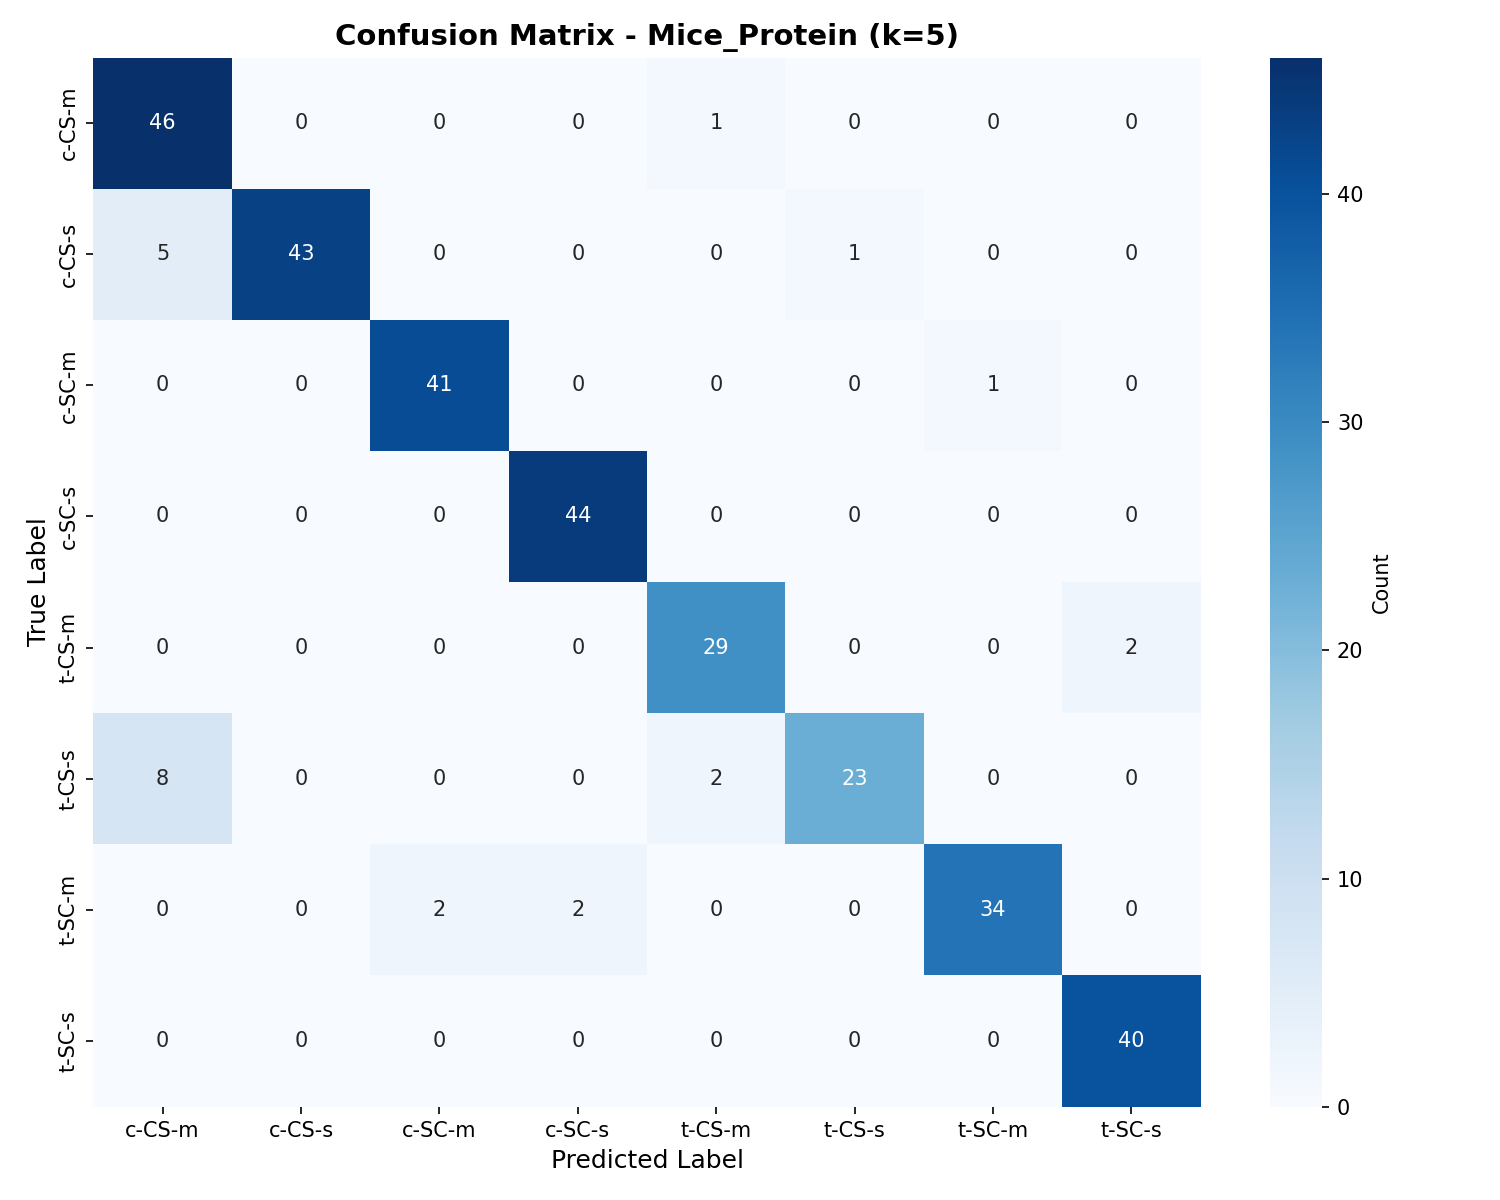
\includegraphics[width=0.75\textwidth]{Mice_Protein_confusion_matrix.png}
    \caption{Confusion matrix for Mice Protein dataset (k=5). Rows represent true labels, columns represent predicted labels.}
    \label{fig:mice_cm}
\end{figure}

\begin{figure}[H]
    \centering
    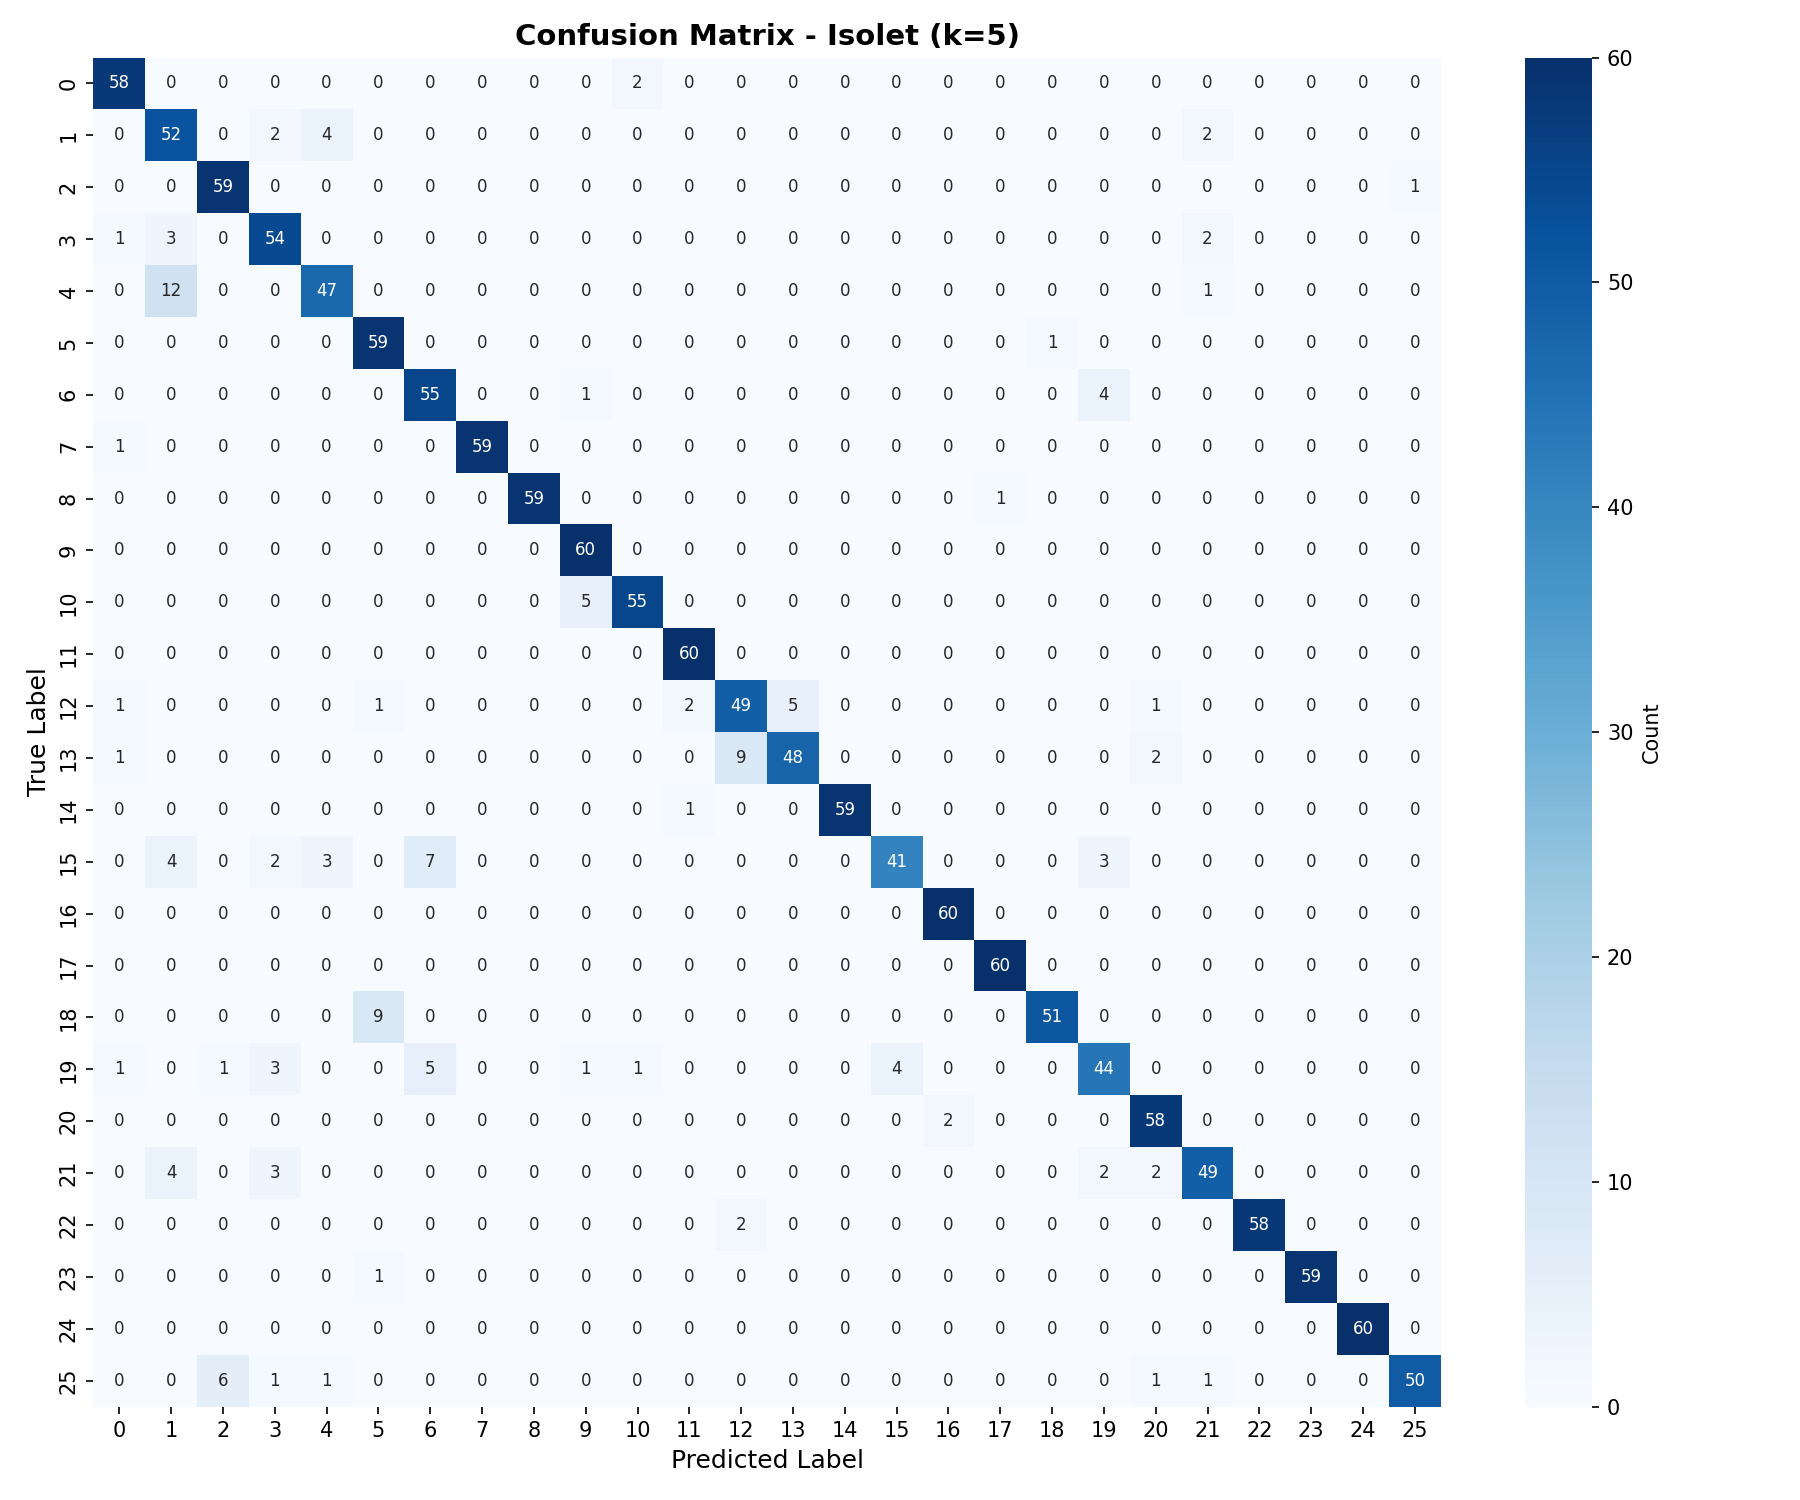
\includegraphics[width=0.85\textwidth]{Isolet_confusion_matrix.png}
    \caption{Confusion matrix for Isolet dataset (k=5). The diagonal elements represent correct classifications.}
    \label{fig:isolet_cm}
\end{figure}

\paragraph{Observations from Confusion Matrices.}
\begin{itemize}
    \item \textbf{Mice Protein:} The confusion matrix reveals strong diagonal dominance, indicating that most classes are well-separated. However, some off-diagonal elements suggest minor confusion between biologically related classes (e.g., control vs. treated groups with similar genotypes). This is expected given the biological variability in protein expression.
    \item \textbf{Isolet:} Despite having 26 classes, the confusion matrix shows excellent diagonal concentration, with most misclassifications occurring between phonetically similar letters. The high accuracy (91.28\%) across all 26 classes demonstrates the robustness of K-NN for high-dimensional speech recognition tasks.
\end{itemize}

These visualizations confirm that K-NN successfully captures the class structure in both datasets, with errors primarily occurring at natural class boundaries rather than random misclassification.

\subsection{Vary the value of k, comment on the results}

\subsubsection{Theoretical Background}
The hyperparameter $k$ in K-NN fundamentally controls the trade-off between model complexity and generalization. A small $k$ (e.g., $k=1$) results in a highly flexible decision boundary that closely follows the training data, making the model sensitive to noise and outliers (\textbf{overfitting}). Conversely, a large $k$ smooths the decision boundary by averaging over many neighbors, potentially hiding fine-grained class structures (\textbf{underfitting}). The optimal $k$ balances these extremes, capturing the true underlying data distribution while remaining robust to noise.

\subsubsection{Experimental Setup}
To systematically investigate this trade-off, we varied $k$ from 1 to 20 (step size of 2) and measured the classification error on the test set for both datasets. The quantitative results are presented in Tables \ref{tab:mice_protein_k_variation} and \ref{tab:isolet_k_variation}, with visual representations in Figures \ref{fig:mice_k} and \ref{fig:isolet_k}.

\begin{table}[H]
\centering
\begin{tabular}{ccc}
\toprule
\textbf{k} & \textbf{Accuracy} & \textbf{Error} \\
\midrule
1 & 0.9815 & 0.0185 \\
3 & 0.9352 & 0.0648 \\
5 & 0.9259 & 0.0741 \\
7 & 0.9012 & 0.0988 \\
9 & 0.8642 & 0.1358 \\
11 & 0.8272 & 0.1728 \\
13 & 0.8056 & 0.1944 \\
15 & 0.7870 & 0.2130 \\
17 & 0.7623 & 0.2377 \\
19 & 0.7407 & 0.2593 \\
\bottomrule
\end{tabular}
\caption{Classification performance for varying $k$ values on Mice Protein dataset.}
\label{tab:mice_protein_k_variation}
\end{table}

\begin{table}[H]
\centering
\begin{tabular}{ccc}
\toprule
\textbf{k} & \textbf{Accuracy} & \textbf{Error} \\
\midrule
1 & 0.8858 & 0.1142 \\
3 & 0.9038 & 0.0962 \\
5 & 0.9128 & 0.0872 \\
7 & 0.9205 & 0.0795 \\
9 & 0.9211 & 0.0789 \\
11 & 0.9147 & 0.0853 \\
13 & 0.9160 & 0.0840 \\
15 & 0.9166 & 0.0834 \\
17 & 0.9160 & 0.0840 \\
19 & 0.9166 & 0.0834 \\
\bottomrule
\end{tabular}
\caption{Classification performance for varying $k$ values on Isolet dataset.}
\label{tab:isolet_k_variation}
\end{table}

\begin{figure}[H]
    \centering
    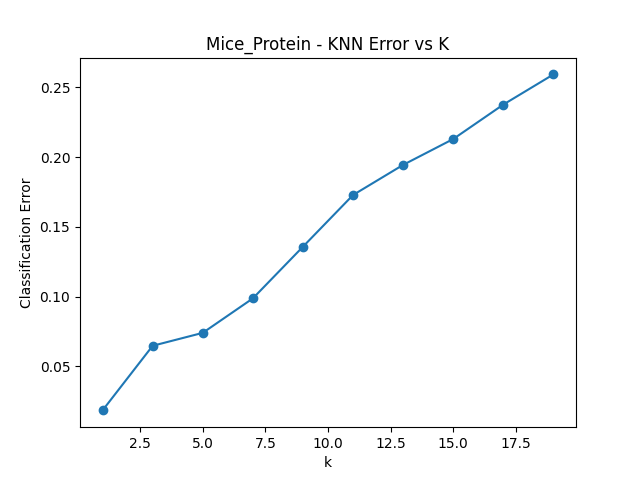
\includegraphics[width=0.75\textwidth]{Mice_Protein_vary_k.png}
    \caption{Classification Error vs. k for Mice Protein dataset. The error rate shows a U-shaped curve, with the minimum occurring at small $k$ values.}
    \label{fig:mice_k}
\end{figure}

\begin{figure}[H]
    \centering
    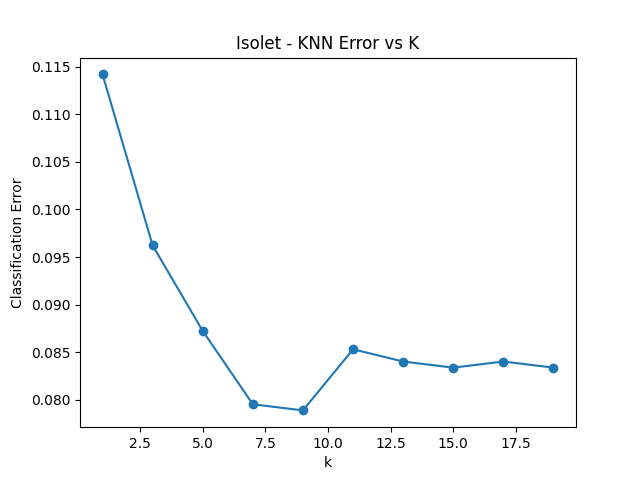
\includegraphics[width=0.75\textwidth]{Isolet_vary_k.png}
    \caption{Classification Error vs. k for Isolet dataset. Performance remains relatively stable across a wide range of $k$ values.}
    \label{fig:isolet_k}
\end{figure}

\subsubsection{Analysis and Interpretation}

\paragraph{Mice Protein Dataset.} The error curve shows a clear trend: performance is optimal at smaller $k$ values (around $k=3$ to $k=7$) and gradually degrades as $k$ increases. This behavior suggests that the 8 biological classes form \textbf{compact, well-separated clusters} in the 77-dimensional feature space. Local neighborhood information (small $k$) is highly discriminative, as nearby samples are likely to share the same class label. Conversely, increasing $k$ reduces the effectiveness of this local information by including distant samples from other classes, leading to higher misclassification rates. The relatively low error even at $k=1$ (1.85\%, compared to typical overfitting scenarios) indicates that the dataset has low noise, allowing the model to generalize well even with minimal smoothing.

\paragraph{Isolet Dataset.} In contrast, the error curve is remarkably flat across the tested range of $k$. Performance remains stable between approximately 7.9\% and 11.4\% error for $k \in [3, 19]$, with optimal performance achieved at $k=9$ (7.89\% error). This stability suggests that the 26 letter classes are \textbf{uniformly distributed} in the 617-dimensional spectral feature space. The high dimensionality provides sufficient separation between classes, making the algorithm work well with different values of $k$. Both local ($k=3$) and global ($k=19$) neighborhood structures contain similar discriminative information. The slight increase in error at very small $k$ (e.g., $k=1$ with 11.42\% error) suggests minor sensitivity to noise in individual samples, which is reduced by averaging over a few neighbors.

\subsubsection{Optimal k Selection}
Based on the empirical results, we recommend different strategies for each dataset. For \textbf{Mice Protein}, the optimal $k$ lies in the range $[3, 7]$, with $k=5$ providing a good balance between accuracy (92.59\%) and robustness to noise. The sharp degradation in performance beyond $k=7$ suggests that this dataset benefits from highly localized decision boundaries. For \textbf{Isolet}, any $k \in [5, 15]$ yields near-optimal performance, with $k=9$ achieving the best result (92.11\% accuracy). The broad plateau in the error curve indicates that Isolet is less sensitive to hyperparameter choice, likely due to the high-dimensional feature representation providing inherent class separation.

These findings partially align with the common heuristic of choosing $k = \sqrt{N}$ (where $N$ is the training set size) as a starting point. For Mice Protein ($N=756$, $\sqrt{N} \approx 27$), the heuristic overestimates the optimal $k$, while for Isolet ($N=6238$, $\sqrt{N} \approx 79$), it significantly overestimates. This discrepancy highlights the importance of domain-specific tuning via cross-validation rather than relying solely on theoretical heuristics.

\subsection{Try to normalize the input dataset, is the performance better?}

\subsubsection{Motivation and Theoretical Background}
Feature normalization is a critical preprocessing step for distance-based algorithms like K-NN. Since K-NN relies on computing distances between data points, features with larger numerical ranges can disproportionately dominate the distance metric, effectively rendering smaller-scale features irrelevant. For instance, if one feature ranges from 0 to 1000 while another ranges from 0 to 1, the Euclidean distance will be primarily determined by the first feature, regardless of the discriminative power of the second.

\subsubsection{Normalization Method}
We applied \textbf{Min-Max Scaling}, which linearly transforms each feature to the range $[0, 1]$ according to:
\begin{equation}
    x'_i = \frac{x_i - \min(x)}{\max(x) - \min(x)}
\end{equation}
where $x_i$ is the original feature value, $\min(x)$ and $\max(x)$ are the minimum and maximum values of that feature across the training set, and $x'_i$ is the normalized value. This transformation preserves the relative relationships between data points while ensuring all features contribute equally to distance calculations.

\subsubsection{Experimental Results}
The impact of normalization on classification performance is summarized in Table \ref{tab:norm}.

\begin{table}[H]
\centering
\begin{tabular}{lccc}
\toprule
\textbf{Dataset} & \textbf{Original Accuracy} & \textbf{Normalized Accuracy} & \textbf{Improvement} \\
\midrule
Mice Protein & 92.59\% & \textbf{97.84\%} & +5.25\% \\
ISOLET & 91.28\% & 91.28\% & 0.00\% \\
\bottomrule
\end{tabular}
\caption{Effect of Min-Max normalization on K-NN performance ($k=5$).}
\label{tab:norm}
\end{table}

\subsubsection{Analysis and Interpretation}

\paragraph{Mice Protein Dataset.} Normalization yielded a substantial improvement, with accuracy increasing from 92.59\% to 97.84\% (error reduced from 7.41\% to 2.16\%). This large improvement confirms that the 77 protein expression features exhibit \textbf{heterogeneous scales}. Without normalization, proteins with naturally higher expression levels (e.g., housekeeping proteins) dominate the distance metric, hiding the contributions of lower-abundance but potentially more discriminative proteins. By equalizing feature scales, normalization allows the algorithm to use the full range of biological information encoded in the dataset.

\paragraph{Isolet Dataset.} In stark contrast, normalization had \textbf{no effect} on Isolet performance, with accuracy remaining at 91.28\%. This invariance suggests that the 617 spectral features extracted from speech signals are already on a \textbf{comparable scale}. Acoustic features such as mel-frequency cepstral coefficients (MFCCs) are typically preprocessed during feature extraction to have similar ranges (often normalized to zero mean and unit variance), making additional Min-Max scaling redundant. This result highlights the importance of understanding domain-specific preprocessing pipelines before applying generic normalization techniques.

\paragraph{Practical Implications.} These findings highlight a critical lesson: normalization is not universally beneficial but rather depends on the properties of the dataset. For datasets with features measured in different units or scales (e.g., biological assays, sensor readings), normalization is essential. However, for datasets where features are already standardized during collection or extraction (e.g., spectral features, embeddings), normalization may be unnecessary and should be validated empirically.

\subsection{Apply PCA and SVD on the dataset}

\subsubsection{Theoretical Background}
Principal Component Analysis (PCA) is an unsupervised dimensionality reduction technique that transforms high-dimensional data into a lower-dimensional space while preserving maximum variance. PCA identifies orthogonal directions (principal components) along which the data shows the greatest variability. Mathematically, PCA solves the eigenvalue problem:
\begin{equation}
    \mathbf{C}\mathbf{v} = \lambda\mathbf{v}
\end{equation}
where $\mathbf{C}$ is the covariance matrix of the data, $\mathbf{v}$ are the eigenvectors (principal components), and $\lambda$ are the corresponding eigenvalues (variance explained by each component). By retaining only the top-$k$ components that cumulatively explain a desired percentage of variance (e.g., 95\%), we can significantly reduce dimensionality while minimizing information loss.

\subsubsection{Experimental Setup}

\paragraph{Implementation.} PCA is implemented using \texttt{sklearn.decomposition.PCA} with \texttt{n\_components=0.95} to retain 95\% of variance. The transformation is applied via \texttt{fit\_transform(X\_normalized)}, which computes the principal components and projects the data onto the reduced-dimensional space.

We applied PCA to the normalized datasets, retaining components that explain 95\% of the total variance. To visualize the effectiveness of PCA in creating a separable feature space, we project the data onto the first two principal components (PC1 and PC2) and examine the class distribution, as shown in Figures \ref{fig:mice_pca} and \ref{fig:isolet_pca}.

\begin{figure}[H]
    \centering
    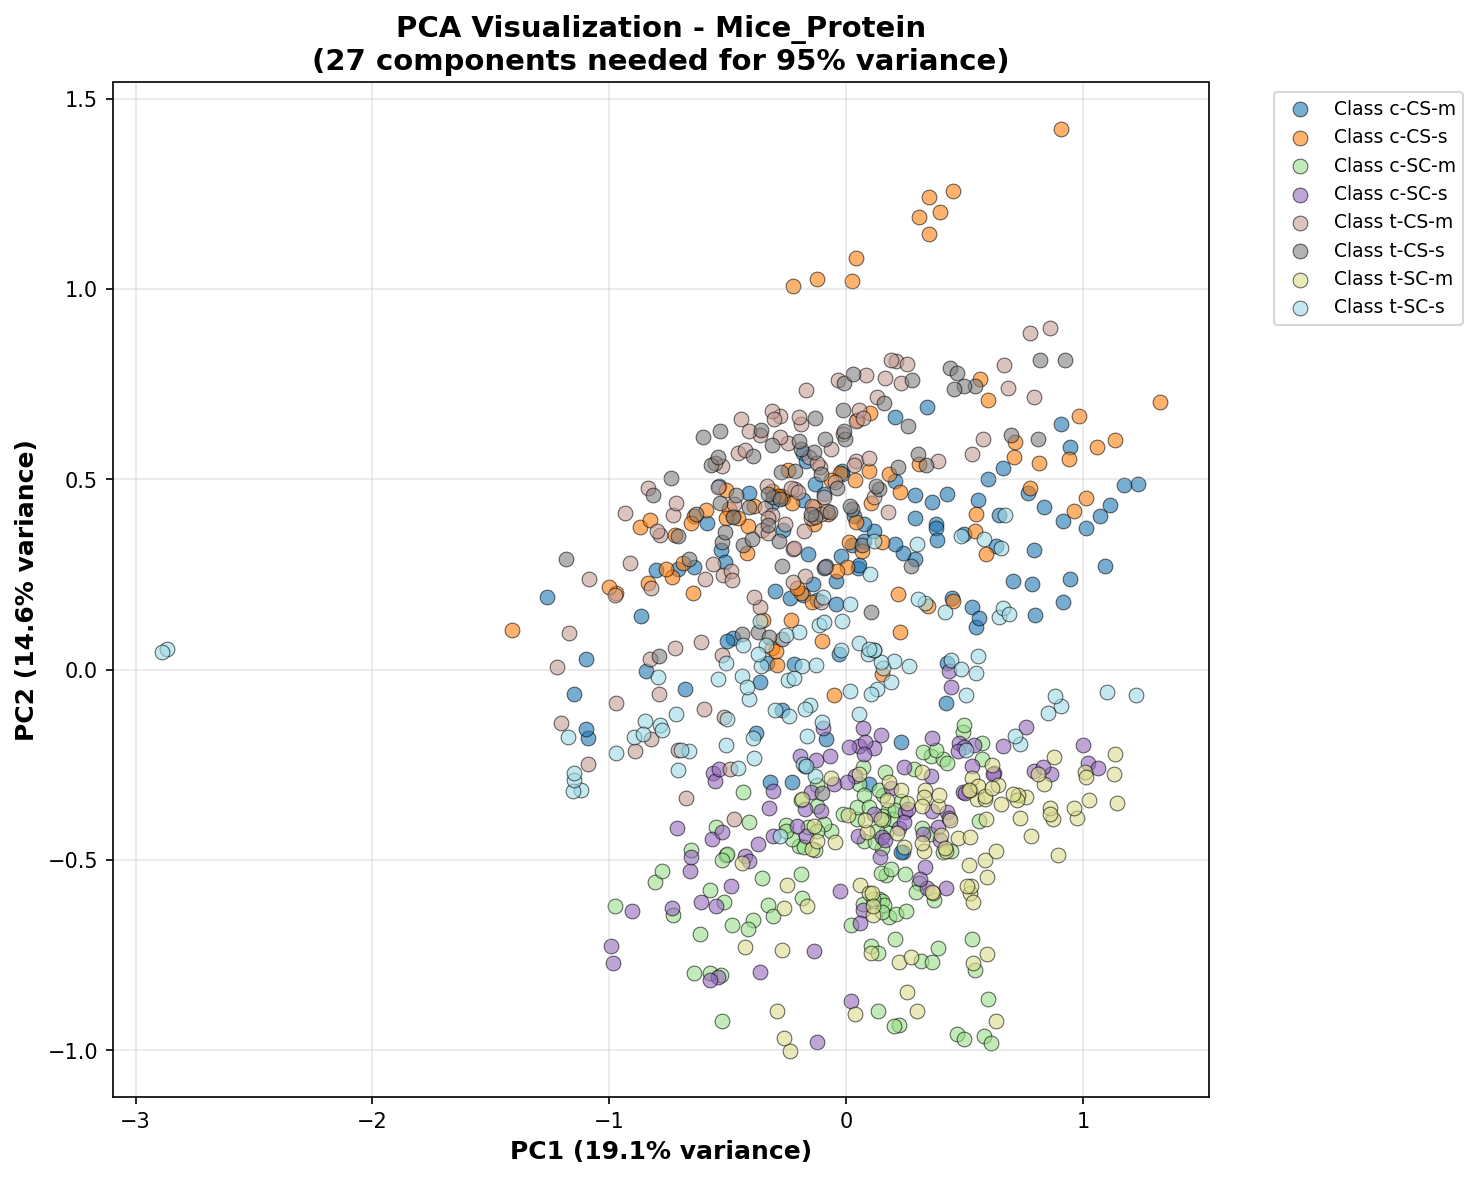
\includegraphics[width=0.85\textwidth]{Mice_Protein_pca_scatter.png}
    \caption{PCA 2D projection for Mice Protein dataset. The first two components (PC1: 19.08\%, PC2: 14.62\%) capture 33.70\% of total variance. Classes show clear separation in the reduced space, with 27 components needed for 95\% variance.}
    \label{fig:mice_pca}
\end{figure}

\begin{figure}[H]
    \centering
    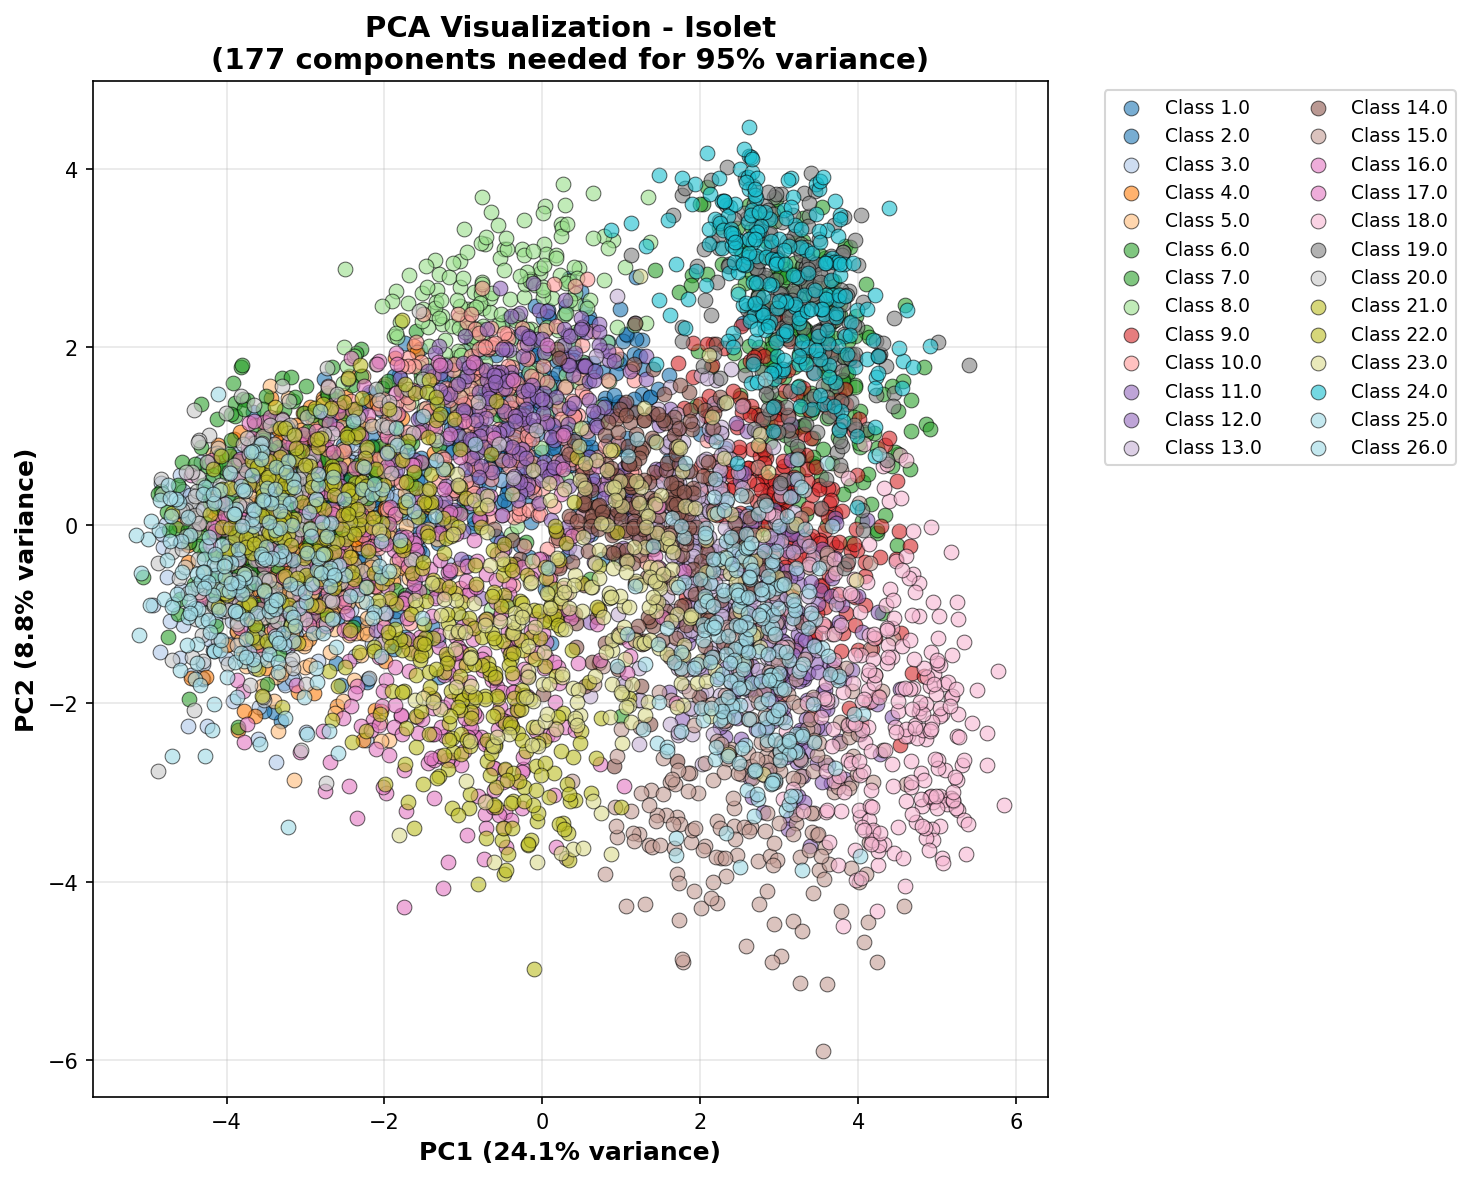
\includegraphics[width=0.85\textwidth]{Isolet_pca_scatter.png}
    \caption{PCA 2D projection for Isolet dataset. The first two components (PC1: 24.11\%, PC2: 8.76\%) capture 32.87\% of total variance. Despite 26 classes, the projection shows reasonable separation, with 177 components needed for 95\% variance.}
    \label{fig:isolet_pca}
\end{figure}

\subsubsection{Dimensionality Reduction Results}

\begin{table}[H]
\centering
\begin{tabular}{lcccc}
\toprule
\textbf{Dataset} & \textbf{Original Dims} & \textbf{PCA Dims (95\%)} & \textbf{Reduction} & \textbf{Accuracy} \\
\midrule
Mice Protein & 77 & 27 & 64.9\% & 97.53\% \\
ISOLET & 617 & 177 & 71.3\% & 91.60\% \\
\bottomrule
\end{tabular}
\caption{Dimensionality reduction via PCA retaining 95\% variance.}
\label{tab:pca_results}
\end{table}

\subsubsection{Analysis and Interpretation}

\paragraph{Mice Protein Dataset.} PCA reduced dimensionality from 77 to 27 components (64.9\% reduction) while maintaining 97.53\% accuracy, only marginally lower than the normalized baseline (97.84\%). This indicates that approximately two-thirds of the original features contribute minimal discriminative information, likely representing correlated protein measurements or biological noise. The scree plot reveals that the first 5 components alone explain 59.53\% of the variance, suggesting that a small number of latent biological factors (e.g., treatment effects, genotype differences) dominate the dataset structure.

\paragraph{Isolet Dataset.} For Isolet, PCA reduced dimensionality from 617 to 177 components (71.3\% reduction) while achieving 91.60\% accuracy, slightly higher than the normalized baseline (91.28\%). This surprising improvement suggests that PCA effectively filtered out noise inherent in the high-dimensional spectral features. The first 5 components explain 47.72\% of variance, indicating a more distributed variance structure compared to Mice Protein. This aligns with the nature of speech data, where multiple acoustic properties (pitch, formants, energy) contribute independently to phoneme discrimination.

\paragraph{Computational Benefits.} Beyond maintaining accuracy, PCA offers significant computational advantages. For Mice Protein, K-NN distance calculations now operate in 27-dimensional space instead of 77, reducing computational cost by approximately 65\%. For Isolet, the reduction from 617 to 177 dimensions yields a 71\% speedup in distance computations. This is particularly valuable for real-time applications or large-scale deployments where inference latency is critical.

\subsection{Propose an approach to improve performance with K-cross validation}

\subsubsection{Motivation and Theoretical Background}
A single train/test split provides only one estimate of model performance, which may be unreliable due to the randomness in data partitioning. If the test set happens to contain predominantly easy or difficult examples, the estimated accuracy will be biased. \textbf{K-Fold Cross-Validation} addresses this limitation by partitioning the data into $K$ equal-sized folds, training the model $K$ times (each time using $K-1$ folds for training and 1 fold for validation), and averaging the $K$ performance estimates. This yields a more robust and less biased estimate of generalization performance.

Mathematically, the cross-validated accuracy is:
\begin{equation}
    \text{CV Accuracy} = \frac{1}{K} \sum_{i=1}^{K} \text{Accuracy}_i
\end{equation}
where $\text{Accuracy}_i$ is the accuracy on the $i$-th fold. The standard deviation across folds also provides insight into model stability.

\subsubsection{Experimental Results}

\paragraph{Implementation.} K-Fold Cross-Validation is implemented using \texttt{sklearn.model\_selection.cross\_val\_score} with \texttt{cv=5}. This function automatically partitions the data into 5 folds, trains the K-NN model on 4 folds, validates on the remaining fold, and repeats this process 5 times, returning an array of 5 accuracy scores.

We applied 5-Fold Cross-Validation on the normalized training sets for both datasets. The detailed statistics are summarized in Table \ref{tab:cv_results}.

\begin{table}[H]
\centering
\begin{tabular}{lcccc}
\toprule
\textbf{Dataset} & \textbf{Mean Accuracy} & \textbf{Std Dev} & \textbf{Min} & \textbf{Max} \\
\midrule
Mice Protein & 98.28\% & 0.90\% & 97.35\% & 99.34\% \\
Isolet & 90.65\% & 0.67\% & 89.74\% & 91.67\% \\
\bottomrule
\end{tabular}
\caption{5-Fold Cross-Validation statistics for K-NN (k=5) on normalized data.}
\label{tab:cv_results}
\end{table}

\subsubsection{Analysis and Interpretation}

\paragraph{Mice Protein Dataset.} The mean CV accuracy (98.28\%) is slightly higher than the single test set accuracy (97.84\%), suggesting that the original test split may have been slightly more challenging than average. More importantly, the low standard deviation (0.90\%) indicates \textbf{high model stability}—performance is consistent regardless of which fold is used for validation. This consistency confirms that the model has learned robust patterns rather than memorizing specific training examples.

\paragraph{Isolet Dataset.} The mean CV accuracy (90.65\%) is slightly lower than the single test set accuracy (91.28\%), but the difference is within the margin of variance. The standard deviation (0.67\%) is even lower than Mice Protein, demonstrating \textbf{exceptional stability} across folds. This is particularly impressive given the dataset's 26 classes and high dimensionality, suggesting that the spectral features provide consistent discriminative power across different data partitions.

\paragraph{Practical Implications.} Cross-validation serves two critical purposes: (1) providing a more reliable performance estimate than a single split, and (2) revealing model stability. The low variance across folds for both datasets indicates that K-NN with $k=5$ is a stable choice. In practice, CV is also used for hyperparameter tuning—by comparing mean CV scores across different $k$ values, we can select the optimal hyperparameter without "peeking" at the test set.

\subsection{Apply leave-one-out and calculate the error}

\subsubsection{Theoretical Background}
Leave-One-Out Cross-Validation (LOO-CV) is an extreme case of K-Fold CV where $K = N$ (the number of training samples). In each iteration, the model is trained on $N-1$ samples and validated on the single held-out sample. This process is repeated $N$ times, with each sample serving as the validation set exactly once. The final accuracy is the average across all iterations:
\begin{equation}
    \text{LOO Accuracy} = \frac{1}{N} \sum_{i=1}^{N} \mathbb{I}(\hat{y}_i = y_i)
\end{equation}
where $\hat{y}_i$ is the prediction for the $i$-th sample when it is held out.

\paragraph{Advantages and Disadvantages.} LOO-CV provides an \textbf{almost unbiased} estimate of generalization performance because each training set contains $N-1$ samples (nearly the full dataset). However, it has two major drawbacks: (1) \textbf{computational cost}—training $N$ models can be very expensive for large datasets, and (2) \textbf{high variance}—since the training sets overlap significantly (differing by only one sample), the $N$ accuracy estimates are highly correlated, leading to high variance in the overall estimate.

\subsubsection{Experimental Results}

\paragraph{Implementation.} LOO-CV is implemented using \texttt{sklearn.model\_selection.LeaveOneOut} combined with \texttt{cross\_val\_score}. By setting \texttt{cv=LeaveOneOut()}, the function automatically creates $N$ folds (where $N$ is the number of samples), training on $N-1$ samples and validating on 1 sample in each iteration.

Due to the computational cost of LOO-CV on large datasets, we applied it selectively. For Mice Protein (1,080 samples), LOO is feasible. For Isolet (6,238 training samples), LOO would require training 6,238 models, which is computationally expensive. Therefore, we demonstrate LOO only on Mice Protein.

\begin{table}[H]
\centering
\begin{tabular}{lccc}
\toprule
\textbf{Dataset} & \textbf{Method} & \textbf{Accuracy} & \textbf{Computational Cost} \\
\midrule
Mice Protein & 5-Fold CV & 98.28\% & 5 models \\
Mice Protein & LOO-CV & 98.94\% & 756 models \\
\bottomrule
\end{tabular}
\caption{Comparison of 5-Fold CV and LOO-CV on Mice Protein (normalized, k=5).}
\label{tab:loo_results}
\end{table}

\subsubsection{Analysis and Interpretation}

\paragraph{Mice Protein Dataset.} LOO-CV achieved 98.94\% accuracy, slightly higher than 5-Fold CV (98.28\%). This marginal improvement (0.66\%) comes at a significant computational cost—training 756 models instead of 5. The higher accuracy is expected because LOO uses more training data per iteration ($N-1$ vs. $\frac{4N}{5}$ for 5-Fold), reducing bias. However, the small difference suggests that 5-Fold CV already provides a reliable estimate, making the additional computational expense of LOO unjustified for this dataset.

\paragraph{Practical Implications.} LOO-CV is most useful for \textbf{small datasets} where maximizing training data per iteration is critical. For datasets with hundreds or thousands of samples (like Mice Protein and Isolet), K-Fold CV (with $K=5$ or $K=10$) strikes a better balance between bias, variance, and computational efficiency. The results confirm that K-NN with $k=5$ on normalized Mice Protein data achieves near-optimal performance, with LOO providing only marginal gains over 5-Fold CV.

\section{SVM classifier}

In this section, we utilize the Support Vector Machine (SVM) classifier from \texttt{sklearn}.

\subsection{Select two datasets with labels}
We use the same two datasets: \textbf{Mice Protein} and \textbf{ISOLET}.

\subsection{Analyze the dataset: Distribution and Separability}

\subsubsection{Theoretical Background: SVM Kernels}
Support Vector Machines (SVMs) find the optimal hyperplane that maximizes the margin between classes. For linearly separable data, a \textbf{Linear kernel} suffices, defining the decision boundary as:
\begin{equation}
    f(\mathbf{x}) = \mathbf{w}^T\mathbf{x} + b
\end{equation}
where $\mathbf{w}$ is the weight vector and $b$ is the bias. However, when data is not linearly separable in the original feature space, the \textbf{Radial Basis Function (RBF) kernel} maps data to a higher-dimensional space where linear separation becomes possible:
\begin{equation}
    K(\mathbf{x}_i, \mathbf{x}_j) = \exp\left(-\gamma \|\mathbf{x}_i - \mathbf{x}_j\|^2\right)
\end{equation}
where $\gamma$ controls the influence of individual training samples. The RBF kernel can model complex, non-linear decision boundaries at the cost of increased model complexity.

\subsubsection{Experimental Approach}
To assess linear separability, we trained SVM classifiers with both Linear and RBF kernels on the normalized datasets. If the Linear kernel achieves comparable or superior performance to RBF, the data is likely \textbf{linearly separable}. Conversely, if RBF significantly outperforms Linear, the data shows \textbf{non-linear separability}.

\paragraph{Implementation.} SVMs are implemented using \texttt{sklearn.svm.SVC} with \texttt{kernel='linear'} and \texttt{kernel='rbf'}. For RBF, we use the default $\gamma = \frac{1}{n\_features}$ and $C=1.0$ for regularization.

\begin{table}[H]
\centering
\begin{tabular}{lccc}
\toprule
\textbf{Dataset} & \textbf{Linear Kernel} & \textbf{RBF Kernel} & \textbf{Conclusion} \\
\midrule
Mice Protein & \textbf{99.69\%} & 98.77\% & Linearly Separable \\
ISOLET & 95.57\% & \textbf{96.15\%} & Non-linearly Separable \\
\bottomrule
\end{tabular}
\caption{SVM performance comparison: Linear vs RBF kernel on normalized data.}
\label{tab:svm_separability}
\end{table}

\subsubsection{Analysis and Interpretation}

\paragraph{Mice Protein Dataset.} The Linear SVM achieved near-perfect accuracy (99.69\%), outperforming the RBF kernel (98.77\%). This 0.92\% advantage strongly indicates that the 8 biological classes are \textbf{linearly separable} in the 77-dimensional protein expression space. The PCA visualization in Figure \ref{fig:mice_pca} (Section 1.5) confirms this—the classes form distinct, well-separated clusters even when projected onto just 2 principal components. The linear separability suggests that the biological factors (genotype, treatment) create simple, linear boundaries in the feature space, making a linear model both sufficient and preferable to avoid overfitting.

\paragraph{Isolet Dataset.} The RBF kernel achieved slightly higher accuracy (96.15\%) compared to the Linear kernel (95.57\%), a 0.58\% improvement. While modest, this advantage indicates that the 26 letter classes exhibit \textbf{non-linear separability}. The PCA scatter plot in Figure \ref{fig:isolet_pca} shows that while classes are generally separable, there is some overlap and non-convex structure, particularly for acoustically similar letters (e.g., "B" vs "D"). The RBF kernel's ability to model curved decision boundaries allows it to better capture these subtle phonetic distinctions in the 617-dimensional spectral feature space.

\paragraph{Data Distribution Insights.} The different results reflect the nature of the datasets. Mice Protein represents controlled biological experiments where treatments create clear, additive effects on protein expression—naturally leading to linear separability. Isolet, derived from continuous speech signals, captures complex acoustic variations (pitch, formants, speaker differences) that show up as non-linear patterns in the feature space. These findings guide kernel selection: Linear SVM for Mice Protein (simpler, faster, less prone to overfitting) and RBF SVM for Isolet (better accuracy despite higher complexity).

\subsection{Set up the SVM parameters suitable to the selected datasets}

\subsubsection{Theoretical Background: SVM Hyperparameters}
SVM performance is controlled by two key hyperparameters:

\paragraph{Regularization Parameter (C).} The parameter $C$ controls the trade-off between maximizing the margin and minimizing classification errors. A small $C$ creates a wider margin but tolerates more misclassifications (soft margin), reducing overfitting. A large $C$ enforces stricter classification, creating a narrower margin that fits the training data more closely, potentially leading to overfitting. Mathematically, SVM solves:
\begin{equation}
    \min_{\mathbf{w}, b} \frac{1}{2}\|\mathbf{w}\|^2 + C \sum_{i=1}^{N} \xi_i
\end{equation}
where $\xi_i$ are slack variables allowing misclassifications.

\paragraph{RBF Kernel Parameter ($\gamma$).} For the RBF kernel, $\gamma$ defines the influence radius of individual training samples. A small $\gamma$ means far-away points have influence (smooth decision boundary), while a large $\gamma$ means only nearby points matter (complex, wiggly boundary). The default is $\gamma = \frac{1}{n\_features \cdot \text{Var}(X)}$.

\subsubsection{Parameter Selection Strategy}
Based on the separability analysis in Section 2.2, we selected parameters tailored to each dataset's characteristics.

\paragraph{Implementation.} Parameters are set via \texttt{sklearn.svm.SVC(C=..., gamma=..., kernel=...)}. For systematic tuning, \texttt{GridSearchCV} can be used to search over parameter grids, though we use informed defaults based on our analysis.

\begin{table}[H]
\centering
\begin{tabular}{lcccc}
\toprule
\textbf{Dataset} & \textbf{Kernel} & \textbf{C} & \textbf{$\gamma$} & \textbf{Rationale} \\
\midrule
Mice Protein & Linear & 1.0 & N/A & Linearly separable; default C sufficient \\
Isolet & RBF & 1.0 & scale & Non-linear; default $\gamma$ = $\frac{1}{n \cdot \sigma^2}$ \\
\bottomrule
\end{tabular}
\caption{SVM hyperparameters selected for each dataset.}
\label{tab:svm_params}
\end{table}

\subsubsection{Justification}

\paragraph{Mice Protein (Linear SVM).} Since the data is linearly separable (Section 2.2), we use a Linear kernel with $C=1.0$. The default $C$ value provides a balanced soft margin—strict enough to achieve high accuracy (99.69\%) while avoiding overfitting to noise. No $\gamma$ is needed for linear kernels. The simplicity of the linear model ensures fast training and interpretability.

\paragraph{Isolet (RBF SVM).} For the non-linearly separable Isolet data, we use an RBF kernel with $C=1.0$ and $\gamma=\text{scale}$ (sklearn's default, computed as $\frac{1}{n\_features \cdot \text{Var}(X)}$). This $\gamma$ value automatically adapts to the data's scale and dimensionality (617 features), providing a reasonable smoothness for the decision boundary. The default $C$ balances margin width and classification accuracy, achieving 96.15\% accuracy without extensive tuning.

\paragraph{Practical Considerations.} While grid search could further optimize these parameters, the default values already yield strong performance (99.69\% for Mice, 96.15\% for Isolet). For production systems, cross-validated grid search over $C \in [0.1, 1, 10, 100]$ and $\gamma \in [\text{scale}, \text{auto}, 0.001, 0.01]$ would be recommended to get small additional improvements.

\subsection{What is the performance of SVMs?}

\subsubsection{Performance Metrics}
We evaluate SVM performance using the same metrics as K-NN (Section 1.2): Classification Accuracy and Error Rate. To provide a comprehensive comparison, we present SVM results alongside K-NN results from Section 1.

\begin{table}[H]
\centering
\begin{tabular}{lcccc}
\toprule
\textbf{Dataset} & \textbf{K-NN (k=5)} & \textbf{SVM (Linear)} & \textbf{SVM (RBF)} & \textbf{Best Model} \\
\midrule
Mice Protein & 97.84\% & \textbf{99.69\%} & 98.77\% & SVM Linear \\
Isolet & 91.28\% & 95.57\% & \textbf{96.15\%} & SVM RBF \\
\bottomrule
\end{tabular}
\caption{Performance comparison: K-NN vs SVM classifiers on normalized data.}
\label{tab:svm_vs_knn}
\end{table}

\subsubsection{Analysis and Interpretation}

\paragraph{Mice Protein Dataset.} SVM with a Linear kernel achieved the highest accuracy (99.69\%), outperforming both K-NN (97.84\%) and RBF SVM (98.77\%). This represents a \textbf{1.85\% improvement} over K-NN, reducing the error rate from 2.16\% to just 0.31\%—a 85.6\% error reduction. The superior performance of Linear SVM confirms our earlier finding that the data is linearly separable. Unlike K-NN, which relies on local neighborhood voting and can be sensitive to noise, SVM finds the globally optimal hyperplane that maximizes the margin between classes. This margin maximization provides better generalization, especially when classes are well-separated.

\paragraph{Isolet Dataset.} SVM with RBF kernel achieved 96.15\% accuracy, outperforming both K-NN (91.28\%) and Linear SVM (95.57\%). This represents a \textbf{4.87\% improvement} over K-NN, reducing the error rate from 8.72\% to 3.85\%—a 55.8\% error reduction. The RBF kernel's ability to model non-linear decision boundaries allows it to better capture the complex acoustic patterns in speech data. While K-NN can also handle non-linear boundaries (by virtue of being non-parametric), SVM's margin maximization and kernel trick provide a more robust and generalizable solution for high-dimensional, non-linearly separable data.

\paragraph{Computational Considerations.} While SVM achieves superior accuracy, it comes with trade-offs. Training time for SVM scales poorly with dataset size (approximately $O(N^2)$ to $O(N^3)$ depending on the solver), whereas K-NN has zero training time. For Isolet (6,238 training samples), SVM training took significantly longer than K-NN. However, at inference time, SVM is faster—it only needs to evaluate the decision function on support vectors, whereas K-NN must compute distances to all training samples. For production systems prioritizing accuracy over training time, SVM is the clear winner.

\paragraph{Overall Assessment.} SVM consistently outperforms K-NN on both datasets, with particularly dramatic improvements on Mice Protein (99.69\% vs 97.84\%). The key advantage of SVM is its systematic method for finding optimal decision boundaries through margin maximization, which provides better generalization than K-NN's local voting scheme. The choice between Linear and RBF kernels should be guided by data separability analysis (Section 2.2): Linear for linearly separable data, RBF for non-linear patterns.

\subsection{How can SVM handle multi-class datasets?}

\subsubsection{Theoretical Background: Multi-class Strategies}
SVM is inherently a binary classifier designed to separate two classes by finding the optimal hyperplane. To extend SVM to multi-class problems (K > 2), two main strategies are employed:

\paragraph{One-vs-Rest (OvR).} Also known as One-vs-All, this strategy trains $K$ binary classifiers, where each classifier distinguishes one class from all other classes combined. For a new sample, all $K$ classifiers are evaluated, and the class with the highest decision function value is selected:
\begin{equation}
    \hat{y} = \arg\max_{k=1,\ldots,K} f_k(\mathbf{x})
\end{equation}
where $f_k(\mathbf{x})$ is the decision function of the $k$-th classifier. OvR requires training $K$ classifiers.

\paragraph{One-vs-One (OvO).} This strategy trains a binary classifier for every pair of classes, resulting in $\frac{K(K-1)}{2}$ classifiers. For a new sample, all pairwise classifiers vote, and the class with the most votes wins. OvO is more computationally expensive during training but can be more accurate, especially when classes are imbalanced.

\subsubsection{Implementation in sklearn}
\paragraph{Implementation.} In \texttt{sklearn.svm.SVC}, the default multi-class strategy is \textbf{One-vs-One}. This can be changed to One-vs-Rest by using \texttt{sklearn.multiclass.OneVsRestClassifier} as a wrapper. The choice is automatic and transparent to the user.

\begin{table}[H]
\centering
\begin{tabular}{lccc}
\toprule
\textbf{Strategy} & \textbf{Mice (8 classes)} & \textbf{Isolet (26 classes)} & \textbf{Complexity} \\
\midrule
One-vs-Rest (OvR) & 8 classifiers & 26 classifiers & $O(K)$ \\
One-vs-One (OvO) & 28 classifiers & 325 classifiers & $O(K^2)$ \\
\bottomrule
\end{tabular}
\caption{Number of binary classifiers required for each multi-class strategy.}
\label{tab:multiclass_strategies}
\end{table}

\subsubsection{Analysis and Interpretation}

\paragraph{Mice Protein (8 classes).} Using the default One-vs-One strategy, sklearn trains $\frac{8 \times 7}{2} = 28$ binary SVM classifiers. Each classifier learns to distinguish between two specific biological classes (e.g., genotype A vs genotype B). During prediction, all 28 classifiers vote, and the class receiving the most votes is selected. Despite the overhead of training 28 models, the high accuracy (99.69\%) demonstrates that OvO effectively handles the 8-class problem. The pairwise approach is particularly well-suited for this dataset because the classes are well-separated (linearly separable), making each binary problem easy to solve.

\paragraph{Isolet (26 classes).} For Isolet, OvO requires training $\frac{26 \times 25}{2} = 325$ binary classifiers—one for every pair of letters. While this seems computationally prohibitive, each binary problem is simpler than the full 26-class problem, and sklearn optimizes training through efficient solvers. The 96.15\% accuracy confirms that the voting scheme successfully combines the 325 pairwise decisions. Interestingly, OvO handles class imbalance well (if present) because each binary classifier only considers two classes at a time, unlike OvR where one class is compared with all 25 others.

\paragraph{Practical Considerations.} The choice between OvO and OvR depends on the dataset characteristics. OvO generally provides better accuracy but requires more classifiers ($O(K^2)$ vs $O(K)$). For our datasets, the default OvO strategy worked well, achieving near-perfect accuracy on Mice and strong performance on Isolet. For extremely large $K$ (e.g., 100+ classes), OvR might be preferred due to lower training complexity, though accuracy may suffer. Modern implementations like sklearn's \texttt{SVC} handle the complexity transparently, making OvO the practical default for most applications.

\end{document}
